%Página
\section{Integridade}

A Integridade diz respeito à precisão e consistência das informações ao longo de seu ciclo de vida. Este pilar assegura que os dados não sejam alterados de forma indevida, seja por erros acidentais ou por ações maliciosas. A integridade é mantida através de mecanismos de verificação, como somas de verificação, assinaturas digitais e funções de hash. Esses métodos permitem que qualquer alteração nos dados seja detectada, garantindo que a informação recebida é exatamente a mesma que foi enviada originalmente, sem modificações não autorizadas.
\subsection{Hash}

Um hash é uma função que transforma uma entrada de dados (que pode variar de alguns bytes a grandes volumes de dados) em uma saída de tamanho fixo, geralmente representada como uma sequência de caracteres alfanuméricos. Esta transformação é determinística, o que significa que a mesma entrada sempre produzirá a mesma saída.\\

Alguns exemplos de algoritmos hash populares incluem a família de algoritmos SHA-2 (Secure Hash Algorithm 2), que inclui SHA-224, SHA-256, SHA-384 e SHA-512. Os algoritmos SHA-2 produzem hashes de diferentes tamanhos, sendo o SHA-256 e o SHA-512 os mais comuns, gerando valores de 256 e 512 bits, respectivamente.\\

A Figura \ref{fig:hash} exemplifica a utilização do algoritmo de hash para verificar a integridade de uma informação enviada de \textbf{Bob} para \textbf{Alice}.\\

\begin{figure}[H]
	\centering
	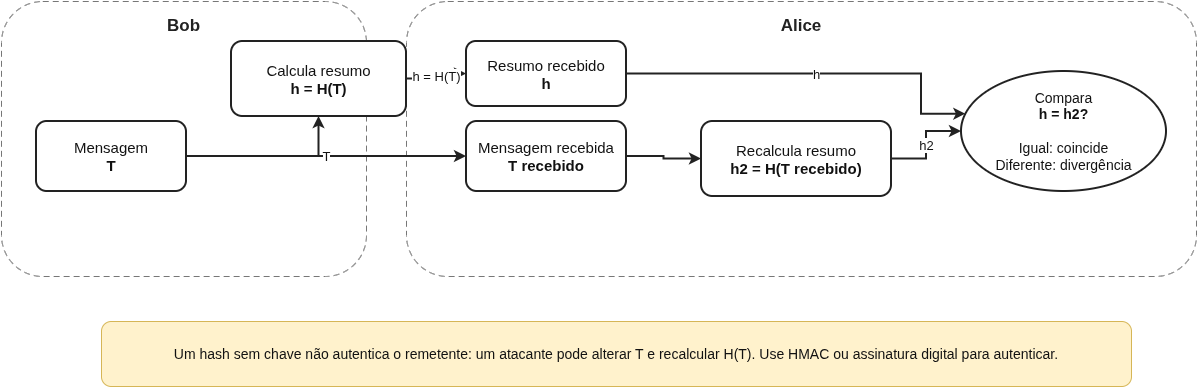
\includegraphics[scale=0.45]{hash.png}
	\caption{Funcionamento do processo de utilização do algoritmo Hash}
	\label{fig:hash}
\end{figure}

Inicialmente, \textbf{Bob} executa o algoritmo de hash sobre a mensagem e obtém o que normalmente é chamado de resumo. Tanto a mensagem quanto o resumo são enviados para \textbf{Alice}. \textbf{Alice} gera novamente o algoritmo de hash sobre a mensagem e compara o resultado do hash com o hash que foi enviado inicialmente por \textbf{Bob}. Se por acaso os valores forem iguais, então isso indica que não houve nenhum tipo de alteração na mensagem.\\

\pagebreak
